\section{Učení s učitelem a evaluace modelů}\label{sec:evaluace}

Tato sekce zavádí společný rámec celého okruhu: co je \emph{učení s~učitelem}, jak rozlišujeme \emph{klasifikaci} a~\emph{regresi}, a~především \textbf{jak model ohodnotíme} -- testovacími daty, křížovou validací a~principem maximum likelihood estimation, a~jakými \emph{metrikami} měříme jeho kvalitu. Konkrétní modely (regrese, stromy, SVM, $\dots$) přijdou v~dalších sekcích; evaluace je společná všem.

\begin{poznamka}[Vztah k~S1]
Okruh S1 (sekce \emph{Strojové učení}) podává učení s~učitelem na úrovni „základní principy``: druhy učení, klasifikace vs.\ regrese, Ockhamova břitva. Zde to nezdvojujeme -- jen krátce zrekapitulujeme a~rovnou jdeme do hloubky, kterou S1 výslovně přenechává okruhu S3 (evaluační metriky, křížová validace).
\end{poznamka}

\subsection{Úlohy učení s učitelem}

\begin{definice}[Učení s~učitelem, klasifikace, regrese]
Při \textbf{učení s~učitelem} máme \emph{trénovací množinu} $N$ příkladů $(\mathbf{x}_i,t_i)$, kde $\mathbf{x}_i\in\mathbb{R}^D$ je vstup (vektor příznaků) a~$t_i$ je \emph{cíl} (požadovaný výstup, label). Hledáme funkci (model) $y$, která dobře předpovídá cíl i~pro \emph{nové, neviděné} vstupy. Podle typu cíle:
\begin{itemize}
  \item \textbf{regrese} -- cíl je reálné číslo, $t\in\mathbb{R}$ (cena, teplota, výnos);
  \item \textbf{klasifikace} -- cíl je jedna z~$K$ tříd, $t\in\{0,1,\dots,K-1\}$ (spam/ham, druh kytky). Model může vracet jen třídu, nebo celé \emph{rozdělení pravděpodobností} tříd.
\end{itemize}
\end{definice}

\begin{intuice}
Příklady chápeme jako nezávislé vzorky z~neznámého \emph{rozdělení generujícího data}. Cílem není zapamatovat trénovací množinu (to je pouhá \emph{optimalizace}), ale \textbf{generalizovat} -- dobře předpovídat data ze stejného rozdělení, která model neviděl. Optimalizace na trénovacích datech je jen prostředek; tím, co nás zajímá, je chyba na nezávislých datech. Celá tato sekce je o~tom, jak takovou chybu \emph{poctivě změřit}.
\end{intuice}

\subsection{Ohodnocení modelu: testovací data, křížová validace, maximum likelihood}

\subsubsection*{Trénovací, validační a~testovací množina}

Chybu na neviděných datech nelze měřit na trénovací množině (model je na ni „naladěn`` a~chybu podhodnotí). Data proto dělíme:
\begin{itemize}
  \item \textbf{trénovací} -- na nich se učí parametry modelu (váhy);
  \item \textbf{validační} (development) -- na nich ladíme \emph{hyperparametry} (např.\ stupeň polynomu, sílu regularizace, $k$ u~$k$-NN) a~rozhodujeme o~\emph{včasném zastavení}; viz sekce~\ref{sec:preuceni};
  \item \textbf{testovací} -- použijí se \emph{jen jednou na konci} k~odhadu generalizační chyby. Kdo ladí podle testovacích dat, klame sám sebe.
\end{itemize}

\begin{definice}[$k$-násobná křížová validace]
Dat je vždy málo na to, vyčlenit velkou validační množinu. \textbf{$k$-násobná křížová validace} ($k$-fold cross-validation) data rozdělí na $k$ stejných dílů (\emph{foldů}). Postupně bere každý díl jako validační a~zbylých $k-1$ dílů jako trénovací; natrénuje a~změří chybu. Výsledný odhad je \emph{průměr} $k$ takto získaných chyb. Využije tak na validaci postupně \emph{všechna} data, ale model nikdy netestuje na datech, na nichž se učil.
\end{definice}

\begin{center}
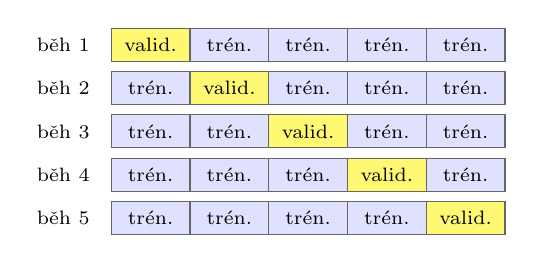
\begin{tikzpicture}[scale=1.0]
  \def\W{1.0} \def\H{0.42} \def\G{0.13}
  \foreach \r [count=\ri] in {0,1,2,3,4}{
    \pgfmathsetmacro\y{0-\r*(\H+\G)}
    \pgfmathsetmacro\yc{\y+\H/2}
    \node[anchor=east,font=\scriptsize] at (-0.15,\yc) {běh~\ri};
    \foreach \c in {0,1,2,3,4}{
      \pgfmathsetmacro\x{\c*\W}
      \pgfmathsetmacro\xc{\x+\W/2}
      \ifnum\c=\r
        \draw[fill=yellow!55,draw=black!60] (\x,\y) rectangle ++(\W,\H);
        \node[font=\scriptsize] at (\xc,\yc) {valid.};
      \else
        \draw[fill=blue!12,draw=black!60] (\x,\y) rectangle ++(\W,\H);
        \node[font=\scriptsize] at (\xc,\yc) {trén.};
      \fi
    }
  }
\end{tikzpicture}
\obrpopis{$5$-násobná křížová validace: data jsou v~$5$ dílech, v~každém z~$5$ běhů slouží jiný díl jako validační (žlutě) a~zbylé čtyři k~trénování (modře). Odhad chyby je průměrem chyb z~pěti běhů. Krajní případ $k=N$ (každý příklad sám fold) se nazývá \emph{leave-one-out}.}
\end{center}

\subsubsection*{Maximum likelihood estimation}

Mnoho modelů (lineární i~logistická regrese, naivní Bayes) se učí \emph{pravděpodobnostně}: model definuje pravděpodobnost dat při daných parametrech a~my hledáme parametry, které pozorovaná data činí \emph{nejvíc pravděpodobnými}.

\begin{definice}[Maximum likelihood estimation (MLE)]
Mějme model s~parametry $\mathbf{w}$, který datům přiřazuje pravděpodobnost (věrohodnost) $p(\text{data}\mid\mathbf{w})$. Při nezávislých příkladech se faktorizuje, $p(\text{data}\mid\mathbf{w})=\prod_{i=1}^N p(t_i\mid \mathbf{x}_i;\mathbf{w})$. \textbf{Maximum likelihood estimation} (maximálně věrohodný odhad) parametrů je
\[ \mathbf{w}_{\mathrm{MLE}} = \argmax_{\mathbf{w}} \prod_{i=1}^N p(t_i\mid \mathbf{x}_i;\mathbf{w}) = \argmin_{\mathbf{w}} \sum_{i=1}^N \big(-\log p(t_i\mid \mathbf{x}_i;\mathbf{w})\big). \]
\end{definice}

\begin{intuice}
Logaritmus mění součin na součet a~je rostoucí, takže maximum nezmění; navíc se lépe počítá a~derivuje. Veličina $-\log p(t_i\mid\mathbf{x}_i;\mathbf{w})$ je \emph{negative log-likelihood} (NLL, záporná logaritmická věrohodnost) a~slouží přímo jako \textbf{ztrátová funkce}: minimalizovat NLL $=$ maximalizovat věrohodnost. Pro normálně rozdělený šum dává MLE přesně \emph{nejmenší čtverce} (sekce~\ref{sec:linreg}), pro klasifikaci \emph{křížovou entropii} (sekce~\ref{sec:logisticka}). Maximum likelihood tak propojuje „intuitivní`` ztrátové funkce s~pravděpodobnostním modelem.
\end{intuice}

\subsection{Evaluační metriky pro klasifikaci}

Základem evaluace binárního klasifikátoru je \textbf{matice záměn} (confusion matrix): tabulka, kolik příkladů které skutečné třídy bylo predikováno do které třídy.

\begin{center}
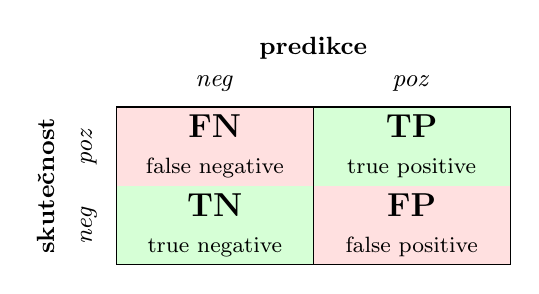
\begin{tikzpicture}[scale=1.0]
  \def\W{2.5} \def\H{1.0}
  % cells
  \fill[green!16] (0,0) rectangle (\W,\H);          % TN
  \fill[red!12]  (\W,0) rectangle (2*\W,\H);         % FP (skut. neg, pred pos)
  \fill[red!12]  (0,\H) rectangle (\W,2*\H);         % FN
  \fill[green!16] (\W,\H) rectangle (2*\W,2*\H);     % TP
  \draw (0,0) grid[step=\W] (2*\W,2*\H); \draw (0,0) rectangle (2*\W,2*\H);
  % cell labels (velká zkratka + malý popisek na druhém řádku, vejde se do buňky)
  \node[align=center] at (1.5*\W,1.5*\H) {\large\textbf{TP}\\[1pt]{\footnotesize true positive}};
  \node[align=center] at (0.5*\W,1.5*\H) {\large\textbf{FN}\\[1pt]{\footnotesize false negative}};
  \node[align=center] at (1.5*\W,0.5*\H) {\large\textbf{FP}\\[1pt]{\footnotesize false positive}};
  \node[align=center] at (0.5*\W,0.5*\H) {\large\textbf{TN}\\[1pt]{\footnotesize true negative}};
  % column headers (predikce) -- bez prefixu "pred." (dimenzi značí tučný titulek "predikce")
  \node[font=\small] at (0.5*\W,2*\H+0.3) {\emph{neg}};
  \node[font=\small] at (1.5*\W,2*\H+0.3) {\emph{poz}};
  \node[font=\small\bfseries] at (\W,2*\H+0.75) {predikce};
  % row headers (skutečnost) -- bez prefixu "skut."
  \node[font=\small,rotate=90] at (-0.35,1.5*\H) {\emph{poz}};
  \node[font=\small,rotate=90] at (-0.35,0.5*\H) {\emph{neg}};
  \node[font=\small\bfseries,rotate=90] at (-0.9,\H) {skutečnost};
\end{tikzpicture}
\obrpopis{Matice záměn binárního klasifikátoru. Zeleně správné predikce (TP, TN), červeně chyby (FP $=$ falešný poplach, FN $=$ přehlédnutí). Z~těchto čtyř čísel se počítají všechny níže uvedené metriky. Pozitivní třída je obvykle ta „zajímavá`` (nemoc, podvod, anomálie).}
\end{center}

\begin{definice}[Metriky binární klasifikace]
Označme TP, TN, FP, FN počty příkladů v~matici záměn. Pak:
\begin{itemize}
  \item \textbf{accuracy} (úspěšnost): podíl správně klasifikovaných,
    \[ \mathrm{acc} = \frac{\mathrm{TP}+\mathrm{TN}}{\mathrm{TP}+\mathrm{TN}+\mathrm{FP}+\mathrm{FN}}. \]
  \item \textbf{precision} (přesnost): podíl skutečně pozitivních mezi predikovanými pozitivními,
    \[ \mathrm{precision} = \frac{\mathrm{TP}}{\mathrm{TP}+\mathrm{FP}}. \]
  \item \textbf{recall} (úplnost), též \emph{sensitivity} a~\emph{true positive rate} (TPR): podíl zachycených ze skutečně pozitivních,
    \[ \mathrm{recall} = \mathrm{TPR} = \frac{\mathrm{TP}}{\mathrm{TP}+\mathrm{FN}}. \]
  \item \textbf{specificity} (specificita), též \emph{true negative rate} (TNR): podíl zachycených ze skutečně negativních,
    \[ \mathrm{specificity} = \mathrm{TNR} = \frac{\mathrm{TN}}{\mathrm{TN}+\mathrm{FP}}. \]
  \item \textbf{F1} (F1 skóre): harmonický průměr precision a~recall,
    \[ F_1 = \frac{2}{\frac{1}{\mathrm{precision}}+\frac{1}{\mathrm{recall}}} = \frac{2\,\mathrm{TP}}{2\,\mathrm{TP}+\mathrm{FP}+\mathrm{FN}}. \]
\end{itemize}
\end{definice}

\begin{intuice}
\emph{Precision} a~\emph{recall} jsou v~napětí: agresivnější klasifikátor (více predikcí „pozitivní``) zvýší recall, ale sníží precision, a~naopak. F1 je vyvažuje jedním číslem; harmonický průměr (na rozdíl od aritmetického) je nízký, je-li \emph{kterákoli} z~obou nízká. Falešný poplach (FP) a~přehlédnutí (FN) mívají \emph{různě velké} náklady (přehlédnutý nádor vs.\ zbytečná biopsie), proto neexistuje jedna „správná`` metrika -- volíme podle úlohy.
\end{intuice}

\begin{poznamka}[Pozor na nevyvážené třídy]
U~silně nevyvážených dat (např.\ $1\,\%$ podvodů) je \emph{accuracy zavádějící}: triviální klasifikátor „vše negativní`` má accuracy $99\,\%$, a~přitom nezachytí jediný podvod. Tam dává smysl sledovat \emph{precision, recall, F1} nebo \emph{AUC}, ne accuracy.
\end{poznamka}

\subsubsection*{ROC křivka a~AUC}

Klasifikátor obvykle vrací \emph{skóre} (např.\ pravděpodobnost pozitivní třídy) a~třídu přiřadí podle \emph{prahu}. Posouváním prahu měníme kompromis mezi TPR a~FPR.

\begin{definice}[ROC křivka, AUC]
\textbf{ROC křivka} (receiver operating characteristic) vynáší pro všechny prahy bod $(\mathrm{FPR},\mathrm{TPR})$, kde $\mathrm{FPR}=\frac{\mathrm{FP}}{\mathrm{FP}+\mathrm{TN}}=1-\mathrm{specificity}$. Diagonála $\mathrm{TPR}=\mathrm{FPR}$ odpovídá náhodnému hádání, levý horní roh $(0,1)$ dokonalému klasifikátoru. \textbf{AUC} (area under curve) je plocha pod ROC křivkou; rovná se pravděpodobnosti, že náhodný pozitivní příklad dostane vyšší skóre než náhodný negativní. AUC${}=1$ je dokonalý, AUC${}=0{,}5$ náhodný klasifikátor.
\end{definice}

\begin{center}
\begin{tikzpicture}
\begin{axis}[width=7.4cm,height=6.2cm,xlabel={FPR $=1-$specificity},ylabel={TPR $=$ recall},
  xmin=0,xmax=1,ymin=0,ymax=1,xtick={0,0.5,1},ytick={0,0.5,1},
  axis lines=left,every axis plot/.append style={thick},clip=false]
  \addplot[name path=roc,blue!60!black,domain=0:1,samples=80]{x^0.32};
  \addplot[name path=diag,black!55,dashed,domain=0:1,samples=2]{x};
  \addplot[blue!12,opacity=0.5] fill between[of=roc and diag];
  \addplot[only marks,mark=*,mark size=1.6pt,red!70!black] coordinates {(0.2,0.597)};
  \node[font=\scriptsize,anchor=west] at (axis cs:0.235,0.5) {práh};
  \node[font=\scriptsize,blue!60!black] at (axis cs:0.55,0.93) {ROC};
  \node[font=\scriptsize,black!55,rotate=33] at (axis cs:0.68,0.55) {náhodné hádání};
  \node[font=\scriptsize] at (axis cs:0.4,0.58) {AUC};
\end{axis}
\end{tikzpicture}
\obrpopis{ROC křivka (modře): každý bod odpovídá jednomu prahu rozhodování. Čím blíž levému hornímu rohu $(0,1)$, tím lepší. Čárkovaná diagonála je náhodné hádání; plocha pod křivkou (AUC) měří kvalitu nezávisle na volbě prahu.}
\end{center}

\subsubsection*{Řešené příklady: matice záměn a~metriky}

\begin{priklad}[SZZ léto 2022 č.~11: Matice konfuze a~specificita]
\szzotazka{léto 2022}{11}{Evaluace binárního klasifikátoru}\par
\textbf{Zadání.} Testovací množina $1000$ příkladů, $50\,\%$ negativních. Klasifikátor má sensitivity $60\,\%$ a~accuracy $70\,\%$. (1)~Napište kompletní matici konfuze. (2)~Vypočtěte specificity.

\smallskip
\textbf{Řešení.} Je $P=500$ pozitivních a~$N=500$ negativních. Sensitivity (recall) $=\mathrm{TP}/P=0{,}6\Rightarrow\mathrm{TP}=300$, $\mathrm{FN}=200$. Accuracy $=(\mathrm{TP}+\mathrm{TN})/1000=0{,}7\Rightarrow\mathrm{TP}+\mathrm{TN}=700$, odtud $\mathrm{TN}=400$ a~$\mathrm{FP}=N-\mathrm{TN}=100$.
\begin{center}
\begin{tabular}{lcc}
\toprule
& predikováno pozitivní & predikováno negativní \\
\midrule
skutečně pozitivní & $\mathrm{TP}=300$ & $\mathrm{FN}=200$ \\
skutečně negativní & $\mathrm{FP}=100$ & $\mathrm{TN}=400$ \\
\bottomrule
\end{tabular}
\end{center}
Specificity $=\dfrac{\mathrm{TN}}{\mathrm{TN}+\mathrm{FP}}=\dfrac{400}{500}=\boxed{0{,}8}=80\,\%$.
\end{priklad}

\begin{priklad}[SZZ podzim 2024 č.~30: Evaluace z~accuracy a~specificity]
\szzotazka{podzim 2024}{30}{Evaluace binárního klasifikátoru}\par
\textbf{Zadání.} Testovací množina má $1000$ příkladů; klasifikátor $400$ označil jako pozitivní a~$600$ jako negativní, s~accuracy $70\,\%$ a~specificity $80\,\%$. Doplňte matici záměn a~spočtěte precision, recall a~F1.

\smallskip
\textbf{Řešení.} Z~predikcí: $\mathrm{TP}+\mathrm{FP}=400$, $\mathrm{TN}+\mathrm{FN}=600$. Z~accuracy $\mathrm{TP}+\mathrm{TN}=0{,}7\cdot 1000=700$. Specificity $\frac{\mathrm{TN}}{\mathrm{TN}+\mathrm{FP}}=0{,}8$. Soustavu vyřeší
\[ \mathrm{TN}=400,\quad \mathrm{FN}=200,\quad \mathrm{TP}=300,\quad \mathrm{FP}=100 \]
(kontrola: $\mathrm{TN}/(\mathrm{TN}+\mathrm{FP})=400/500=0{,}8$ \faCheck, $(\mathrm{TP}+\mathrm{TN})/1000=0{,}7$ \faCheck). Pak
\[ \text{precision}=\tfrac{300}{400}=\boxed{0{,}75},\quad \text{recall}=\tfrac{300}{500}=\boxed{0{,}6},\quad F_1=\tfrac{2\cdot 0{,}75\cdot 0{,}6}{0{,}75+0{,}6}=\boxed{0{,}\overline{6}}. \]
\end{priklad}

\begin{priklad}[SZZ jaro 2023 č.~7: Matice záměn ze sensitivity a~specificity]
\szzotazka{jaro 2023}{7}{Evaluace binárního klasifikátoru}\par
\textbf{Zadání.} Klasifikátor má sensitivity $0{,}8$ a~specificity $0{,}9$; testováno na $10\,000$ příkladech, z~nichž $500$ je pozitivních. (1)~Spočtěte matici záměn. (2)~Vstup je predikován jako pozitivní -- jaká je pravděpodobnost, že je skutečně pozitivní? (3)~Jaká je accuracy?

\smallskip
\textbf{Řešení.} (1)~Pozitivních je $500$, negativních $9500$. Sensitivity (recall) $=\mathrm{TP}/500=0{,}8\Rightarrow \mathrm{TP}=400$, $\mathrm{FN}=100$. Specificity $=\mathrm{TN}/9500=0{,}9\Rightarrow \mathrm{TN}=8550$, $\mathrm{FP}=950$.
\[ \mathrm{TP}=400,\ \mathrm{FN}=100,\ \mathrm{FP}=950,\ \mathrm{TN}=8550. \]
(2)~Hledaná pravděpodobnost je právě \emph{precision}: $\text{precision}=\frac{400}{400+950}=\frac{400}{1350}\approx\boxed{0{,}296}$. (Ač má klasifikátor vysokou sensitivity, kvůli vzácnosti pozitivní třídy je jen $\sim\!30\,\%$ predikovaných pozitivních skutečně pozitivních -- ukázka, jak nevyváženost sráží precision.) (3)~$\mathrm{acc}=\frac{400+8550}{10000}=\boxed{0{,}895}$.
\end{priklad}

\begin{priklad}[SZZ léto 2023 č.~6: ROC a~precision v~jednom bodě]
\szzotazka{léto 2023}{6}{Testování binárního klasifikátoru}\par
\textbf{Zadání.} Testovací sada má $100$ pozitivních a~$400$ negativních příkladů. (a)~ROC křivka prochází bodem $\mathrm{TPR}=\mathrm{FPR}=20\,\%$; spočtěte precision v~tomto bodě. (b)~Jiný klasifikátor má konstantní $\text{precision}=50\,\%$; znázorněte jeho ROC křivku.

\smallskip
\textbf{Řešení.} (a)~$\mathrm{TPR}=0{,}2\Rightarrow \mathrm{TP}=0{,}2\cdot 100=20$; $\mathrm{FPR}=0{,}2\Rightarrow \mathrm{FP}=0{,}2\cdot 400=80$. Precision $=\frac{20}{20+80}=\boxed{0{,}2}$.

(b)~Konstantní precision $\frac{\mathrm{TP}}{\mathrm{TP}+\mathrm{FP}}=\tfrac12$ znamená $\mathrm{FP}=\mathrm{TP}$ při každém prahu. Protože $\mathrm{TPR}=\frac{\mathrm{TP}}{100}$ a~$\mathrm{FPR}=\frac{\mathrm{FP}}{400}=\frac{\mathrm{TP}}{400}$, platí $\mathrm{FPR}=\tfrac{1}{4}\mathrm{TPR}$, tj.\ $\mathrm{TPR}=4\cdot\mathrm{FPR}$. ROC je tedy \emph{úsečka} z~$(0,0)$ do $(\mathrm{FPR},\mathrm{TPR})=(0{,}25,\,1)$ (při $\mathrm{TPR}=1$ je $\mathrm{FP}=\mathrm{TP}=100$, $\mathrm{FPR}=100/400=0{,}25$).
\begin{center}
\begin{tikzpicture}[scale=2.5]
  \draw[osa] (0,0) -- (1.08,0) node[right,font=\scriptsize]{FPR};
  \draw[osa] (0,0) -- (0,1.12) node[above,font=\scriptsize]{TPR};
  \foreach \t in {0.25,0.5,1}{\draw (\t,0.01)--(\t,-0.01) node[below,font=\tiny]{\t}; \draw (0.01,\t)--(-0.01,\t) node[left,font=\tiny]{\t};}
  \draw[black!45,dashed] (0,0)--(1,1);
  \draw[very thick,blue!60!black] (0,0)--(0.25,1);
  \fill[red!70!black] (0.25,1) circle (0.5pt) node[above right,font=\tiny]{$(0{,}25,\,1)$};
\end{tikzpicture}
\obrpopis{ROC křivka klasifikátoru s~konstantní precision $50\,\%$ na datech $100\!:\!400$: úsečka $\mathrm{TPR}=4\,\mathrm{FPR}$ od počátku do $(0{,}25,1)$. Leží nad diagonálou (lepší než náhoda).}
\end{center}
\end{priklad}

\begin{priklad}[SZZ podzim 2025 č.~28: Dva nástroje na detekci anomálií]
\szzotazka{podzim 2025}{28}{Evaluace binárního klasifikátoru}\par
\textbf{Zadání.} $10\,000$ instancí, z~nichž $1\,\%$ ($100$) jsou anomálie (pozitivní), $9\,900$ normálních. Nástroj~1: accuracy $99{,}5\,\%$, zachytí $90\,\%$ anomálií. Nástroj~2: zachytí $81\,\%$ anomálií, $10\,\%$ nahlášených je falešně pozitivních. Spočtěte matice záměn a~metriky a~rozhodněte, který nástroj zvolit.

\smallskip
\textbf{Řešení.}

\textbf{Nástroj 1.} Recall $0{,}9\Rightarrow \mathrm{TP}=90$, $\mathrm{FN}=10$. Správně klasifikováno $0{,}995\cdot 10000=9950$, z~toho $\mathrm{TN}=9950-90=9860$, takže $\mathrm{FP}=9900-9860=40$.
\[ \text{precision}=\tfrac{90}{130}\approx 0{,}69,\quad \text{recall}=0{,}9,\quad F_1\approx 0{,}78,\quad \mathrm{acc}=0{,}995. \]

\textbf{Nástroj 2.} Recall $0{,}81\Rightarrow \mathrm{TP}=81$, $\mathrm{FN}=19$. „$10\,\%$ nahlášených falešně pozitivních`` znamená $\text{precision}=0{,}9=\frac{\mathrm{TP}}{\mathrm{TP}+\mathrm{FP}}$, odkud $\mathrm{FP}=\tfrac{81}{9}=9$, $\mathrm{TN}=9900-9=9891$.
\[ \text{precision}=0{,}9,\quad \text{recall}=0{,}81,\quad F_1\approx 0{,}85,\quad \mathrm{acc}=0{,}9972. \]

\textbf{Závěr.} Nástroj~2 je lepší ve všech metrikách kromě recall ($0{,}81$ vs.\ $0{,}9$). Hlásí mnohem méně falešných poplachů (FP $9$ vs.\ $40$), takže neobtěžuje správce. Naopak nástroj~1 odhalí víc anomálií; jsou-li kritické, může se i~přes nižší precision vyplatit. Jednoznačná odpověď neexistuje, rozhoduje cena FP vs.\ FN.

\smallskip
\noindent\footnotesize V~původním PDF jsou u~nástroje~2 drobné nekonzistence (zaměněný vzorec precision, „$80$ ze $100$`` místo $81$ a~hodnota $\mathrm{FP}$ označená jako $\mathrm{FN}$); zde uvádíme spočítanou konzistentní variantu, viz též poznámka ve fragmentu v~\texttt{priklady/}.
\end{priklad}

\begin{priklad}[SZZ podzim 2023 č.~31: Metriky a~detekce podvodů]
\szzotazka{podzim 2023}{31}{Evaluační metriky}\par
\textbf{Zadání (zkráceně).} (1)~Definujte accuracy, recall, precision, F1. (2)~Detekce podvodných plateb, kde z~milionů jen stovky jsou podvody -- jaké metriky (ne)použít? (3)~Systém~A: recall $0{,}99$, precision $0{,}2$; systém~B: recall $0{,}9$, precision $0{,}95$. Co znamenají a~který zvolit?

\smallskip
\textbf{Řešení.} (1)~Viz definice výše. (2)~Data jsou silně nevyvážená, proto \emph{accuracy je nevhodná} (triviální „vše legitimní`` má accuracy $\approx 100\,\%$). Vhodné jsou \emph{precision a~recall} (případně F1 nebo AUC), které se soustředí na vzácnou pozitivní třídu. (3)~Systém~A odhalí $99\,\%$ podvodů, ale jen $20\,\%$ jeho hlášení jsou skutečné podvody (oproti B zhruba $5\times$ víc hlášení k~prošetření: $0{,}99/0{,}2\approx 4{,}95$ vs.\ $0{,}9/0{,}95\approx 0{,}95$ na jeden podvod). Systém~B odhalí $90\,\%$ podvodů a~$95\,\%$ hlášení sedí. Pokud nás trápí náklady na prošetřování a~obtěžování zákazníků, volíme \emph{B}; pokud je prioritní zachytit i~poslední podvod, volíme \emph{A}. Jednoznačná odpověď neexistuje, rozhoduje argumentace (cena FP vs.\ FN).
\end{priklad}

\subsection{Evaluační metriky pro regresi}

U~regrese měříme \emph{velikost chyby} predikce $\hat{t}_i=y(\mathbf{x}_i)$ vůči cíli $t_i$.

\begin{definice}[Metriky regrese]
\[ \mathrm{MSE}=\frac1N\sum_i (t_i-\hat t_i)^2,\quad \mathrm{RMSE}=\sqrt{\mathrm{MSE}},\quad \mathrm{MAE}=\frac1N\sum_i |t_i-\hat t_i|. \]
RMSE je ve stejných jednotkách jako cíl; oproti MAE \emph{víc penalizuje velké chyby} (kvadrát). Koeficient determinace $R^2=1-\frac{\sum_i (t_i-\hat t_i)^2}{\sum_i (t_i-\bar t)^2}$ udává podíl rozptylu cíle vysvětlený modelem ($R^2=1$ dokonale, $R^2=0$ jako predikce průměrem).
\end{definice}

\subsection{Naivní Bayesův klasifikátor}

\begin{poznamka}[Nad rámec požadavků]
Naivní Bayes není v~požadavcích jmenován, ale je to standardní pravděpodobnostní klasifikátor probíraný v~NPFL129 (vedle $k$-NN) a~objevuje se v~reálné SZZ otázce; uvádíme ho proto jako řešený příklad klasifikace.
\end{poznamka}

\begin{definice}[Naivní Bayesův klasifikátor]
Pro vstup s~příznaky $x_1,\dots,x_D$ přiřadíme třídu $c$ podle \emph{aposteriorní} pravděpodobnosti (Bayesova věta):
\[ P(c\mid x_1,\dots,x_D)=\frac{P(c)\,P(x_1,\dots,x_D\mid c)}{P(x_1,\dots,x_D)}\;\propto\; P(c)\,P(x_1,\dots,x_D\mid c). \]
\textbf{Naivní} předpoklad je \emph{podmíněná nezávislost} příznaků při dané třídě, takže sdruženou věrohodnost rozložíme na součin:
\[ \hat c=\argmax_{c}\; P(c)\prod_{j=1}^{D} P(x_j\mid c). \]
Pravděpodobnosti $P(c)$ (apriorní třídy) a~$P(x_j\mid c)$ odhadneme z~trénovacích dat relativními četnostmi (MLE). Jmenovatel $P(x_1,\dots,x_D)$ je stejný pro všechny třídy, takže pro výběr maxima stačí čitatel.
\end{definice}

\begin{intuice}
„Naivnost`` je v~předpokladu, že příznaky jsou při dané třídě \emph{nezávislé} -- to skoro nikdy přesně neplatí (např.\ déšť a~oblíbená přednáška spolu mohou korelovat), ale klasifikátor i~tak často dobře funguje a~potřebuje málo dat. Bez tohoto předpokladu bychom museli odhadovat celé sdružené rozdělení $P(x_1,\dots,x_D\mid c)$, což je exponenciálně mnoho parametrů.
\end{intuice}

\begin{priklad}[SZZ jaro 2023 č.~16: Naivní Bayes -- půjde student do školy?]
\szzotazka{jaro 2023}{16}{Naivní Bayesovský klasifikátor}\par
\textbf{Zadání.} Z~$13$ pozorování (atributy \emph{Vstanu}, \emph{Oblíbená přednáška?}, \emph{Počasí}; cíl \emph{Jdu do školy}) určete naivním Bayesem, zda student půjde do školy, jestliže \emph{vstane pozdě}, \emph{nemá oblíbenou přednášku} a~\emph{prší}.
\begin{center}\small
\begin{tabular}{ccccc}
\toprule
Den & Vstanu & Oblíbená přednáška? & Počasí & Jdu do školy\\
\midrule
1 & Brzo & Ne & Slunce & Ne\\
2 & Normálně & Ne & Déšť & Ne\\
3 & Brzo & Ne & Slunce & Ano\\
4 & Pozdě & Ne & Slunce & Ano\\
5 & Pozdě & Ano & Slunce & Ano\\
6 & Pozdě & Ano & Déšť & Ne\\
7 & Brzo & Ano & Déšť & Ano\\
8 & Normálně & Ne & Slunce & Ne\\
9 & Normálně & Ano & Slunce & Ano\\
10 & Pozdě & Ano & Slunce & Ano\\
11 & Normálně & Ano & Déšť & Ano\\
12 & Brzo & Ne & Déšť & Ano\\
13 & Brzo & Ano & Slunce & Ano\\
\bottomrule
\end{tabular}
\end{center}

\smallskip
\textbf{Řešení.} Z~$13$ dnů jde do školy $9\times$ (Ano), nejde $4\times$ (Ne): $P(\text{Ano})=\tfrac{9}{13}$, $P(\text{Ne})=\tfrac{4}{13}$. Spočteme podmíněné četnosti potřebných hodnot:
\[
\begin{aligned}
&P(\text{Pozdě}\mid\text{Ano})=\tfrac{3}{9},\ P(\text{obl}{=}\text{Ne}\mid\text{Ano})=\tfrac{3}{9},\ P(\text{Déšť}\mid\text{Ano})=\tfrac{3}{9};\\
&P(\text{Pozdě}\mid\text{Ne})=\tfrac{1}{4},\ P(\text{obl}{=}\text{Ne}\mid\text{Ne})=\tfrac{3}{4},\ P(\text{Déšť}\mid\text{Ne})=\tfrac{2}{4}.
\end{aligned}
\]
Skóre (čitatel) pro obě třídy:
\[ \text{Ano}:\ \tfrac{9}{13}\cdot\tfrac13\cdot\tfrac13\cdot\tfrac13=\tfrac{1}{39}\approx 0{,}0256,\qquad \text{Ne}:\ \tfrac{4}{13}\cdot\tfrac14\cdot\tfrac34\cdot\tfrac24=\tfrac{3}{104}\approx 0{,}0288. \]
Větší je skóre třídy \emph{Ne}, takže naivní Bayes predikuje, že student \textbf{do školy nepůjde} (po normalizaci $P(\text{Ne}\mid\text{data})\approx 53\,\%$, $P(\text{Ano}\mid\text{data})\approx 47\,\%$ -- těsné). Zajímavé je, že přestože „chodí do školy`` je apriorně mnohem častější, kombinace tří příznaků (pozdě, bez oblíbené přednášky, déšť) převáží ve prospěch „nejde``.
\end{priklad}

\subsection{Praktický postup: od dat k modelu}

Úloha nemusí mířit na jeden algoritmus, ale na \emph{celý postup}: rozpoznat typ úlohy, zvolit model, předzpracovat data, vybrat metriku. Následující reálná otázka SZZ takový postup procvičuje -- nejde o~samostatné téma požadavků, ale o~syntézu pojmů této sekce (a~modelů z~dalších sekcí).

\begin{priklad}[SZZ podzim 2025 č.~29: Predikce z~tabulárních dat]
\szzotazka{podzim 2025}{29}{Predikce pomocí tabulárních dat}\par
\textbf{Zadání (zkráceně).} Zemědělský dataset (pH, srážky, teplota, typ hnojiva, odrůda, velikost farmy, zavlažování, nadm.\ výška) má předpovídat \emph{výnos} (t/ha). (1)~Typ úlohy? (2)~Vhodný model a~proč? (3)~Předzpracování a~zacházení s~typy příznaků. (4)~Evaluační metriky?

\smallskip
\textbf{Řešení.} (1)~\emph{Regrese} s~učitelem -- cíl (výnos) je spojité číslo a~máme trénovací data s~cílovými hodnotami. (2)~Pro tabulární data s~mixem číselných i~kategorických příznaků jsou typicky nejlepší \emph{stromové ansámbly} -- \emph{random forest} nebo \emph{gradient boosting} (XGBoost/LightGBM): zvládnou nelinearity i~interakce, nevyžadují škálování (viz sekce~\ref{sec:kombinace}). Lineární regrese nebo MLP fungují s~pečlivějším předzpracováním. (3)~\emph{Kategorické} příznaky (typ hnojiva, odrůda, zavlažování) zakódovat \emph{one-hot}; \emph{číselné} (pH, srážky, $\dots$) zkontrolovat odlehlé hodnoty a~u~modelů citlivých na škálu \emph{standardizovat}; chybějící hodnoty doplnit (průměr/medián, resp.\ modus). (4)~\emph{MAE}, (R)MSE, případně $R^2$.
\end{priklad}
